\documentclass{beamer}
\usepackage{listings}
\usepackage{graphicx}
\usepackage{caption}
\usepackage{subcaption}
\usepackage{polski}
\usepackage[utf8]{inputenc}
\title{Znajdywanie najkrótszej drogi w grafie - metoda Dijkstry}
\author{Igor Nowicki}
\date{\today}
\institute{WIT - Wyższa Szkoła Informatyki Stosowanej i Zarządzania}
\usetheme{Warsaw}
\begin{document}
\begin{frame}
	\titlepage
\end{frame}
\section{Wstęp}
\subsection{Opis problemu}

\begin{frame}
	Dany jest graf ważony krawędziowo o nieujemnych wagach.

	\begin{figure}
			\centering
			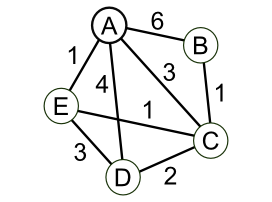
\includegraphics[width=0.4\linewidth]{i00.png}


	\end{figure}

	\pause
	Jaki jest minimalny koszt przejścia pomiędzy wybranymi dwoma węzłami grafu?
\pause
Czy możemy znaleźć stowarzyszoną z tym kosztem optymalną trasę?

\end{frame}

\section{Opis rozwiązania}
\subsection{Opis słowny algorytmu}
\begin{frame}
	Metoda Dijkstry wykorzystuje \emph{zachłanne} podejście do problemu - na każdym kroku ustalamy koszty alternatywnych ścieżek i wybieramy tę o najniższej wartości.
	\pause

	\bigskip
	Algorytm możemy opisać następująco:
	\begin{enumerate}
		\pause
		\item Wybierz nieodwiedzony jeszcze węzeł o najniższej przypisanej wartości.
		      \pause
		\item Zaktualizuj wartości sąsiadów - jeśli ich przypisana wartość jest wyższa, zastąp ją sumą bieżącego węzła i drogi. Zapamiętaj skąd wyszło połączenie.
		      \pause
		\item Powtarzaj kroki 1 i 2 dopóki nie zostaną odwiedzone wszystkie węzły.
	\end{enumerate}
\end{frame}

\subsection{Schemat blokowy}
\begin{frame}
	Schemat blokowy:
	\pause
	\begin{figure}
		\centering
		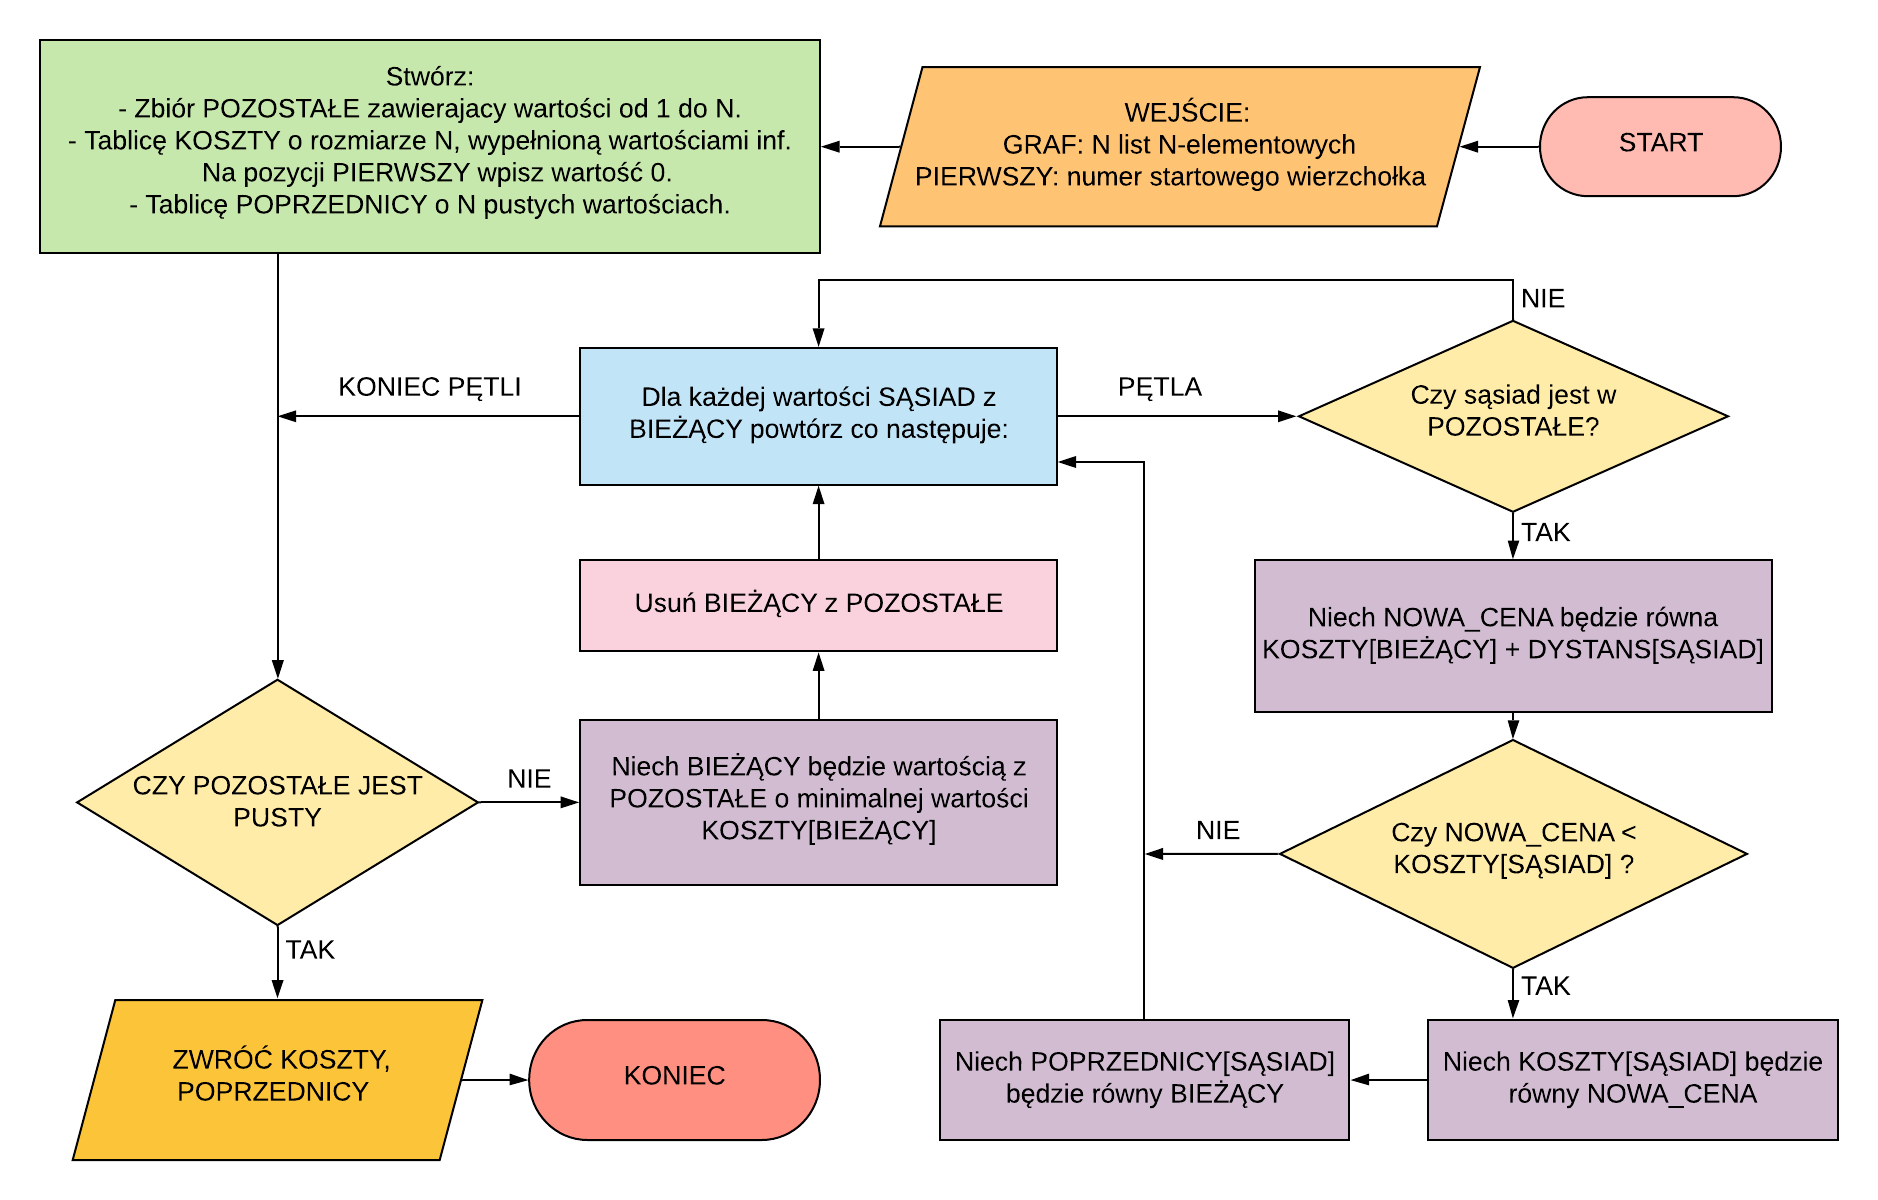
\includegraphics[width=1\linewidth]{flowchart1.png}
	\end{figure}
\end{frame}

\section{Symulacja}

\begin{frame}
	Weźmiemy graf z początku prezentacji:
	\begin{figure}
			\centering
			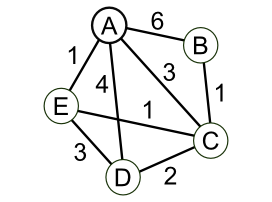
\includegraphics[width=0.5\linewidth]{i00.png}
	
	\end{figure}
	\pause
	Będziemy poszukiwać optymalnych tras z punktu A. Jako test bojowy sprawdzimy, czy algorytm poprawnie znajduje najniższy koszt przejścia z A do B.
\end{frame}
\begin{frame}
	\begin{figure}
		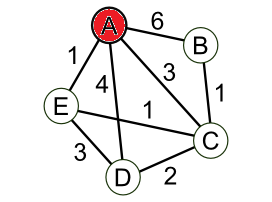
\includegraphics[width=.30\linewidth]{step0.png}
	\end{figure}


	\begin{table}[]


		\begin{tabular}{|l|l|l|l|l|l|}
			\hline
			            & A & B        & C        & D        & E        \\ \hline
			POZOSTAŁE   & + & +        & +        & +        & +        \\ \hline
			KOSZTY      & \only<1>{$\infty$}\only<2>{0}  & $\infty$ & $\infty$ & $\infty$ & $\infty$ \\ \hline
			POPRZEDNICY & - & -        & -        & -        & -        \\ \hline
		\end{tabular}
	\end{table}



	Inicjalizacja. Wszystkie węzły traktujemy jako nieodwiedzone. Bieżący koszt dotarcia do każdego z węzłów jest nieskończony, poza węzłem A, z którego zaczynamy.
\end{frame}
\begin{frame}
	\begin{figure}
		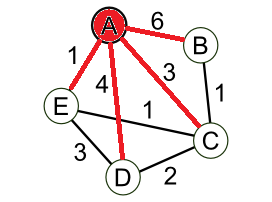
\includegraphics[width=.30\linewidth]{step1.png}
	\end{figure}
	\begin{table}[]
		\begin{tabular}{|l|l|l|l|l|l|}
			\hline
			            & A & B & C & D & E \\ \hline
			POZOSTAŁE   & \alt<2->{-}{+} & + & + & + & + \\ \hline
			KOSZTY      & 0 & \alt<3->{6}{$\infty$} & \alt<3->{3}{$\infty$} & \alt<3->{4}{$\infty$} & \alt<3->{1}{$\infty$} \\ \hline
			POPRZEDNICY & - & \alt<3->{A}{-} & \alt<3->{A}{-} & \alt<3->{A}{-} & \alt<3->{A}{-} \\ \hline
		\end{tabular}
	\end{table}
	Pierwszy krok. Kasujemy A ze zbioru POZOSTAŁE. Uzupełniamy koszty B, C, D oraz E, ustawiamy ich poprzednika na A.
	Ustalamy E jako bieżący węzeł o najniższej wartości z jeszcze nieodwiedzonych.
\end{frame}

\begin{frame}
	\begin{figure}
		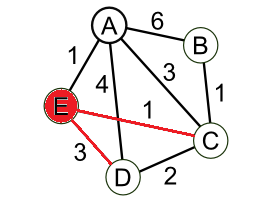
\includegraphics[width=.30\linewidth]{step2.png}
	\end{figure}
	\begin{table}[]
		\begin{tabular}{|l|l|l|l|l|l|}
			\hline
			            & A & B & C & D & E \\ \hline
			POZOSTAŁE   & - & + & + & + & \alt<2->{-}{+} \\ \hline
			KOSZTY      & 0 & 6 & \alt<3->{2}{3} & 4 & 1 \\ \hline
			POPRZEDNICY & - & A & \alt<3->{E}{A} & A & A \\ \hline
		\end{tabular}
	\end{table}
	Drugi krok. Kasujemy E z listy pozostałych, aktualizujemy wartości połączeń z C oraz D. C jest kolejną wartością.
\end{frame}
\begin{frame}
	\begin{figure}
		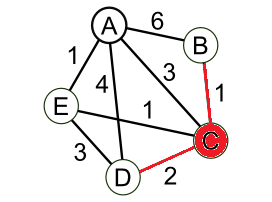
\includegraphics[width=.30\linewidth]{step3.png}
	\end{figure}
	\begin{table}[]
		\begin{tabular}{|l|l|l|l|l|l|}
			\hline
			            & A & B & C & D & E \\ \hline
			POZOSTAŁE   & - & + & \alt<2->{-}{+} & + & - \\ \hline
			KOSZTY      & 0 & \alt<3->{3}{6} & 2 & 4 & 1 \\ \hline
			POPRZEDNICY & - & \alt<3->{C}{A} & E & A & A \\ \hline
		\end{tabular}
	\end{table}
	Trzeci krok. Kasujemy C z pozostałych, aktualizujemy koszty dróg do B oraz D. Następcą będzie B.
\end{frame}
\begin{frame}
	\begin{figure}
		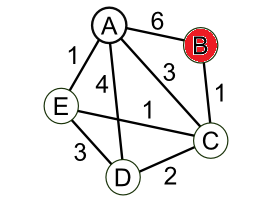
\includegraphics[width=.30\linewidth]{step4.png}
	\end{figure}
	\begin{table}[]
		\begin{tabular}{|l|l|l|l|l|l|}
			\hline
			            & A & B & C & D & E \\ \hline
			POZOSTAŁE   & - & \alt<2->{-}{+} & - & + & - \\ \hline
			KOSZTY      & 0 & 3 & 2 & 4 & 1 \\ \hline
			POPRZEDNICY & - & C & E & A & A \\ \hline
		\end{tabular}
	\end{table}
	Czwarty krok. Usuwamy B z listy pozostałych. Nie aktualizujemy żadnych dróg. Następnym węzłem będzie D.
\end{frame}

\begin{frame}
	\begin{figure}
		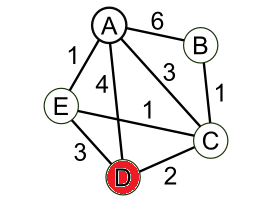
\includegraphics[width=.30\linewidth]{step5.png}
	\end{figure}
	\begin{table}[]
		\begin{tabular}{|l|l|l|l|l|l|}
			\hline
			            & A & B & C & D & E \\ \hline
			POZOSTAŁE   & - & - & - & \alt<2->{-}{+} & - \\ \hline
			KOSZTY      & 0 & 3 & 2 & 4 & 1 \\ \hline
			POPRZEDNICY & - & C & E & A & A \\ \hline
		\end{tabular}
	\end{table}
	Piąty krok. Usuwamy D z listy pozostałych. Ponieważ wszystkie możliwe węzły zostały już uwzględnione, nie aktualizujemy żadnych ścieżek. Algorytm zwraca wyniki i kończy zadanie.
\end{frame}

\begin{frame}
	\begin{table}[]
		\begin{tabular}{|l|l|l|l|l|l|}
			\hline
			            & A & B & C & D & E \\ \hline
			KOSZTY      & 0 & 3 & 2 & 4 & 1 \\ \hline
			POPRZEDNICY & - & C & E & A & A \\ \hline
		\end{tabular}
	\end{table}

Dostaliśmy dwie tablice wyników: KOSZTY i POPRZEDNICY. Na podstawie tego możemy wyczytać, że najniższy koszt podróży z A do B wynosi 3 i następuje według trasy:

$$A\rightarrow E\rightarrow C\rightarrow B.$$

\begin{figure}
	\centering
	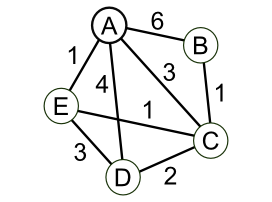
\includegraphics[width=0.3\linewidth]{i00.png}

\end{figure}

\end{frame}

\section{Implementacja}

\begin{frame}
Zaimplementujemy teraz ten algorytm w Pythonie (wersja 3.8).

\begin{figure}
	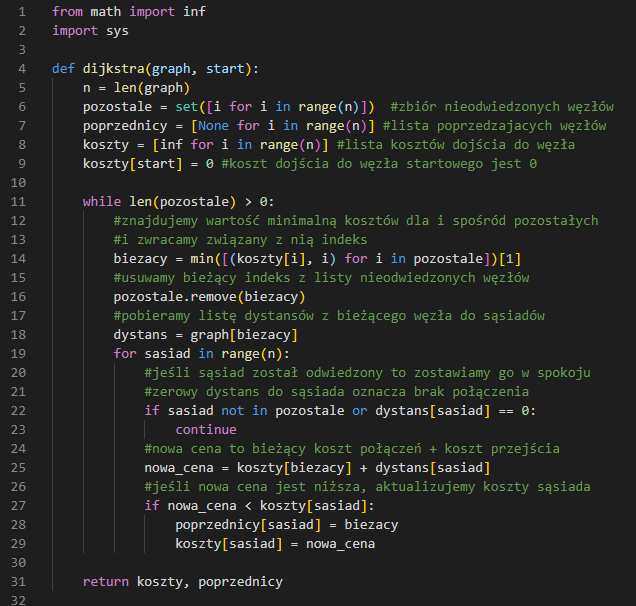
\includegraphics[height=6.8cm]{python.png}
\end{figure}

\end{frame}

\subsection{Szacowanie złożoności czasowej}
\begin{frame}
Oszacowanie złożoności czasowej:

\begin{figure}
\centering
\alt<2->{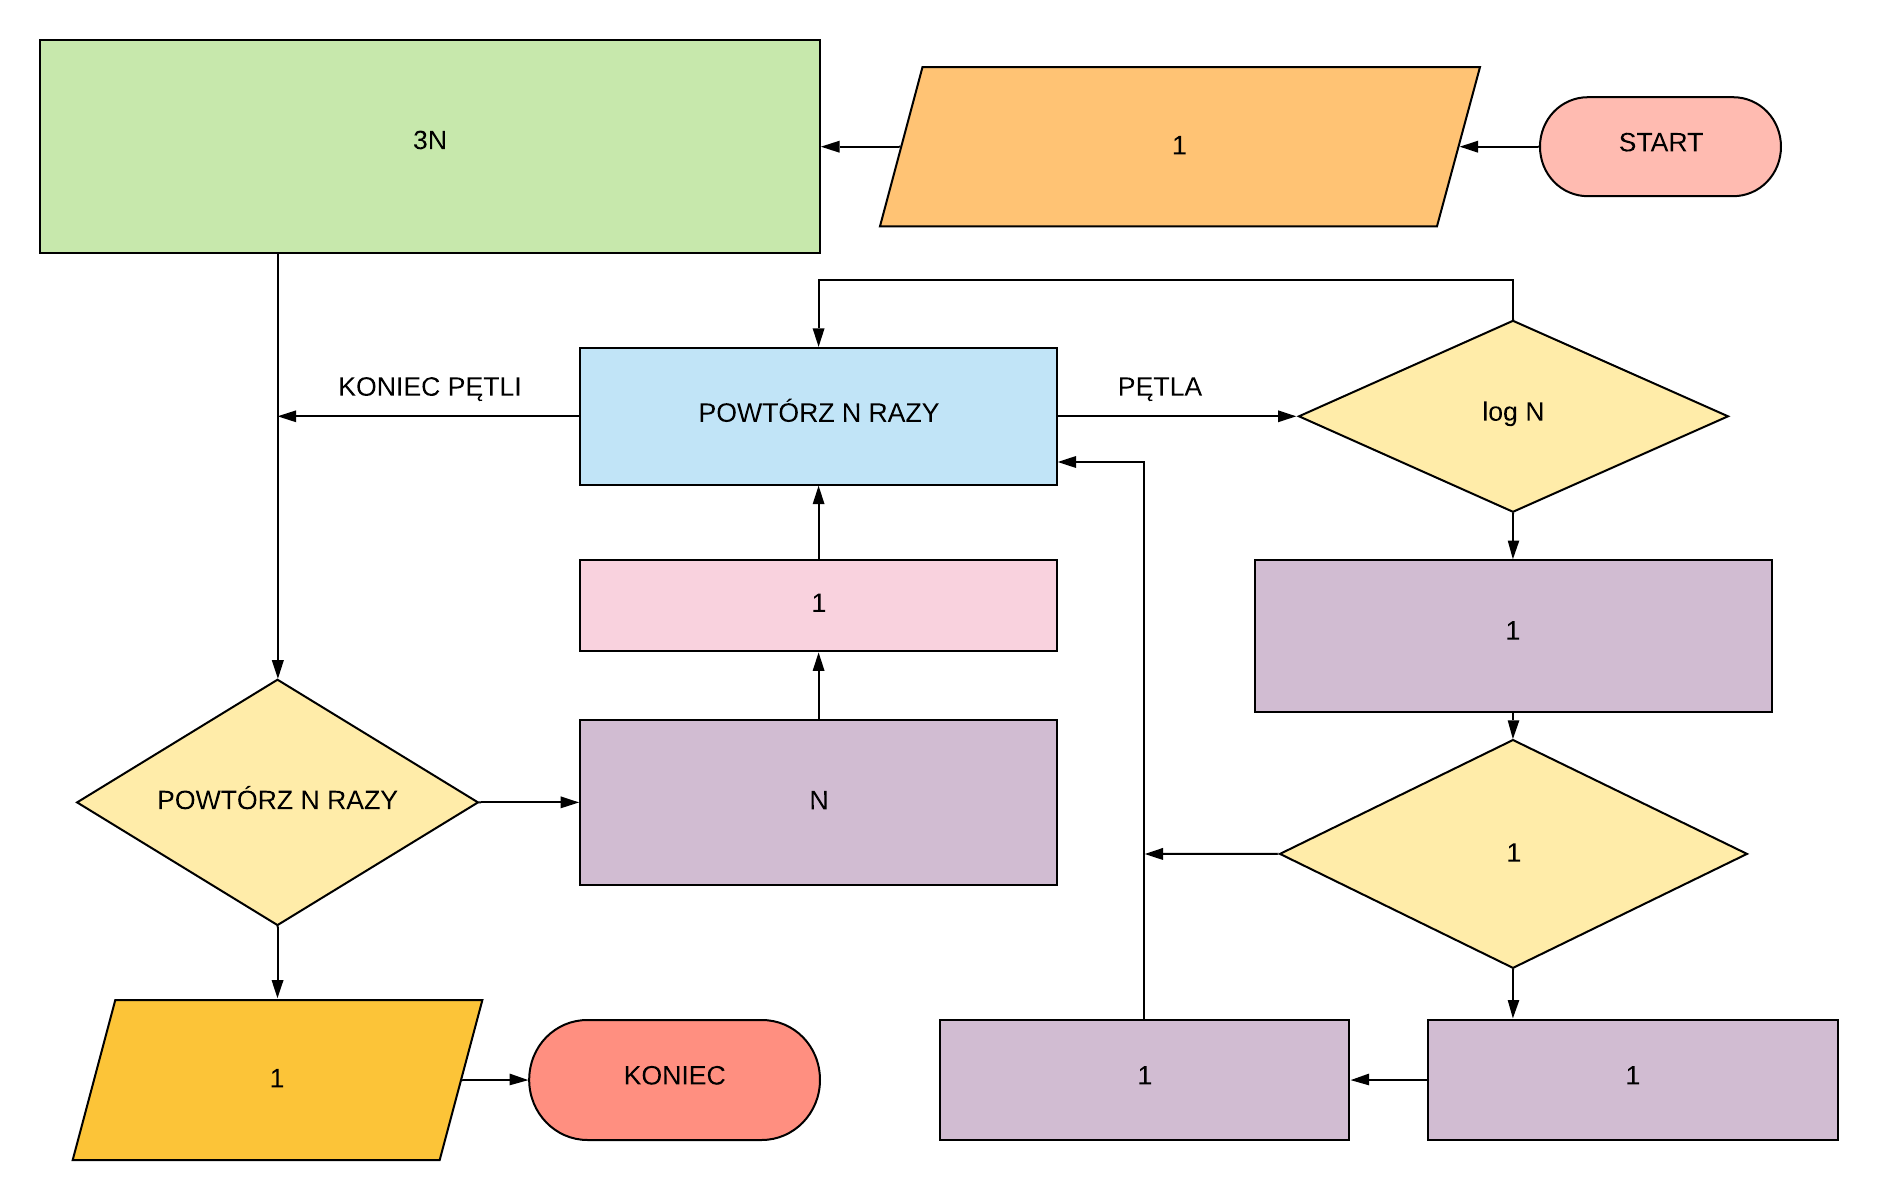
\includegraphics[width=0.7\linewidth]{flowchart2.png}}{
	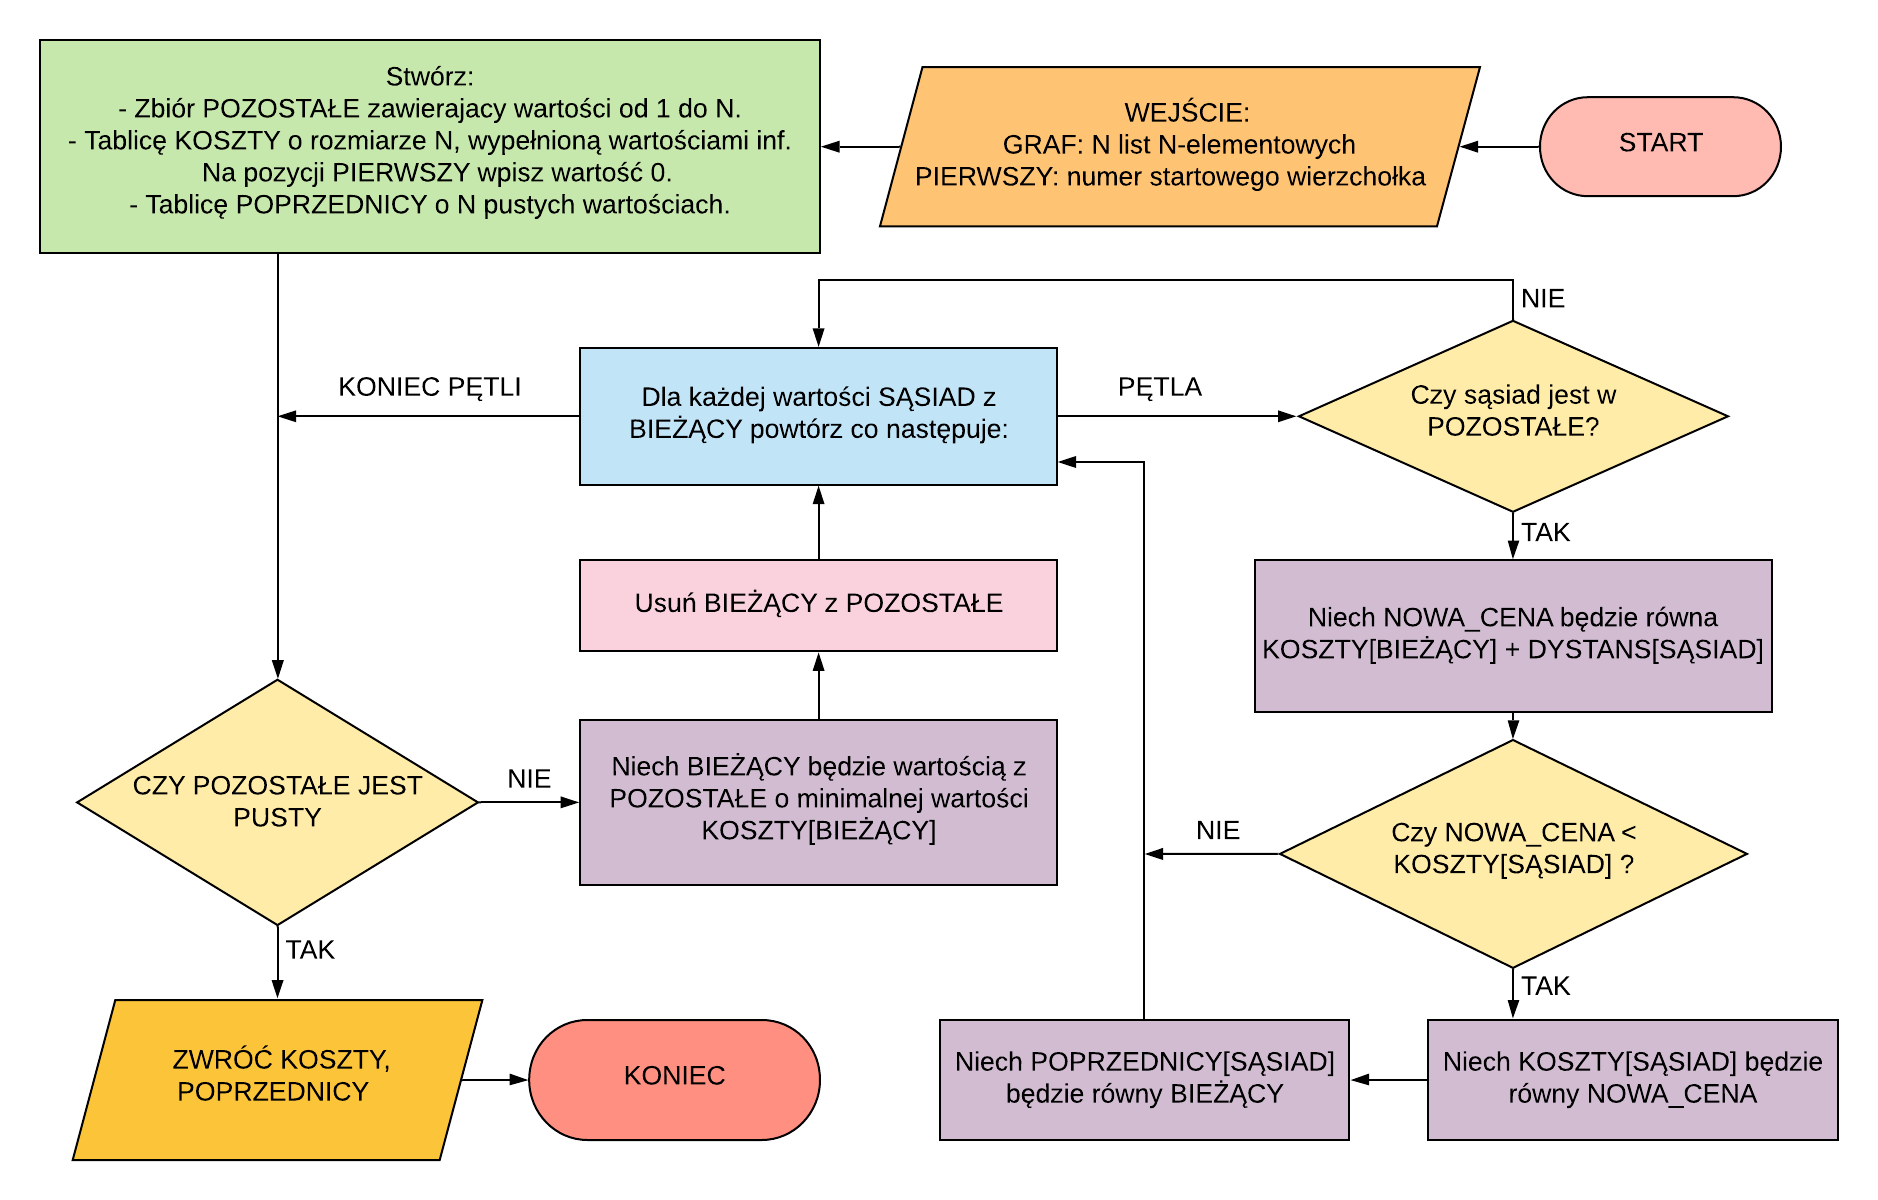
\includegraphics[width=0.7\linewidth]{flowchart1.png}}
\end{figure}
\only<3>{$$T(N) = 1+3N+N\cdot\Big(N+1+N\cdot\big(\log(N) + 1+1+1+1\big)\Big)+1$$}
\only<4>{$$T(N) = 2+4N+5N^2 + N^2\log(N)$$}
\only<5>{$$T(N) \approx O\Big(N^2\log(N)\Big)$$}
\end{frame}

\subsection{Wyznaczanie doświadczalne złożoności czasowej}
\begin{frame}

	Przedstawiona złożoność na wykresie:

	\begin{figure}
\centering
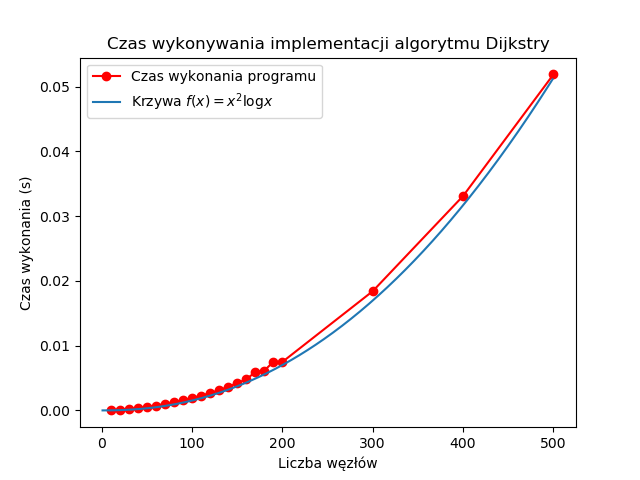
\includegraphics[width=0.8\linewidth]{plot.png}
	\end{figure}

\end{frame}

\begin{frame}
	\Huge\center
	Dziękuję za uwagę!
\end{frame}

\end{document}
